% !TEX root = ../main.tex
\begin{tikzpicture}[line width=1pt,node distance=14mm ,main/.style = {draw, rectangle},scale=1] 

    \node[scale=.8] at (3.15,6){$\textup{Match}[b,\{x_4\}]$};
       
       \node[main] at (3.15,4.5) (9) {
   \begin{tikzpicture}[line width=1pt,node distance=14mm ,main/.style = {draw, circle},scale=1] 
   \node[main,color=black] at (1,1) (x2) {\texttt{$x_2$}};
       \node[main,color=black] at (0,0) (x3) {\texttt{$x_3$}};
       \node[main,fill=blue!40!white,densely dashed] at (1,0) (x4) {\texttt{$x_4$}};
      \draw (x2) -- (x3);
      \draw (x3) -- (x4);
   \end{tikzpicture}
       };
       
    \node[scale=.8] at (-1.5,1.5){$\textup{Match}[c,\{x_4\}]$};
       \node[main] at (-1.5,0) (8) {
   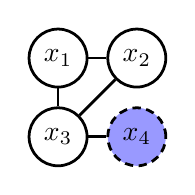
\begin{tikzpicture}[line width=1pt,node distance=14mm ,main/.style = {draw, circle},scale=1] 
   \node[main,color=black] at (0,1) (x1) {\texttt{$x_1$}};
   \node[main,color=black] at (1,1) (x2) {\texttt{$x_2$}};
       \node[main,color=black] at (0,0) (x3) {\texttt{$x_3$}};
       \node[main,fill=blue!40!white,densely dashed] at (1,0) (x4) {\texttt{$x_4$}};
      \draw (x1) -- (x2);
       \draw (x1) -- (x3);
      \draw (x2) -- (x3);
      \draw (x3) -- (x4);
   \end{tikzpicture}
   };
   
    \node[scale=.8] at (1.3,1.5){$\textup{Match}[c,\{x_4\}\cup \{x_1\}]$};
   \node[main] at (1.3,0) (8) {
   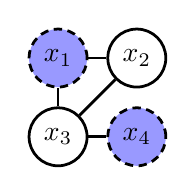
\begin{tikzpicture}[line width=1pt,node distance=14mm ,main/.style = {draw, circle},scale=1] 
   \node[main,fill=blue!40!white,densely dashed] at (0,1) (x1) {\texttt{$x_1$}};
   \node[main,color=black] at (1,1) (x2) {\texttt{$x_2$}};
       \node[main] at (0,0) (x3) {\texttt{$x_3$}};
       \node[main,fill=blue!40!white,densely dashed] at (1,0) (x4) {\texttt{$x_4$}};
      \draw (x1) -- (x2);
       \draw (x1) -- (x3);
      \draw (x2) -- (x3);
      \draw (x3) -- (x4);
   \end{tikzpicture}
   };
   
    \node[scale=.8] at (4.5,1.5){$\textup{Match}[c,\{x_4\}\cup \{x_1,x_2\}]$};
   \node[main] at (4.5 ,0) (8) {
   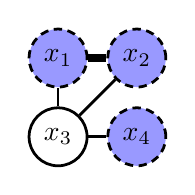
\begin{tikzpicture}[line width=1pt,node distance=14mm ,main/.style = {draw, circle},scale=1] 
   \node[main,fill=blue!40!white,densely dashed] at (0,1) (x1) {\texttt{$x_1$}};
   \node[main,fill=blue!40!white,densely dashed] at (1,1) (x2) {\texttt{$x_2$}};
       \node[main,color=black] at (0,0) (x3) {\texttt{$x_3$}};
       \node[main,fill=blue!40!white,densely dashed] at (1,0) (x4) {\texttt{$x_4$}};
      \draw [line width = 3pt, color=black]  (x1) -- (x2);
       \draw (x1) -- (x3);
      \draw (x2) -- (x3);
      \draw (x3) -- (x4);
   \end{tikzpicture}
   };

   \node[scale=.8] at (7.8,1.5){$\textup{Match}[c,\{x_4\}\cup \{x_1,x_3\}]$};
   \node[main] at (7.8,0) (8) {
   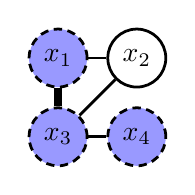
\begin{tikzpicture}[line width=1pt,node distance=14mm ,main/.style = {draw, circle},scale=1] 
   \node[main,fill=blue!40!white,densely dashed] at (0,1) (x1) {\texttt{$x_1$}};
   \node[main,color=black] at (1,1) (x2) {\texttt{$x_2$}};
       \node[main,fill=blue!40!white,densely dashed] at (0,0) (x3) {\texttt{$x_3$}};
       \node[main,fill=blue!40!white,densely dashed] at (1,0) (x4) {\texttt{$x_4$}};
      \draw (x1) -- (x2);
       \draw [line width = 3pt, color=black] (x1) -- (x3);
      \draw (x2) -- (x3);
      \draw (x3) -- (x4);
   \end{tikzpicture}
   };
   
       \draw [decorate,decoration={brace,amplitude=10}] (-1.5,2.5) -- (7.8,2.5) node [black,midway,xshift=-0.6cm] {};
   
       %\node[text width=6cm] at (2,-2){$\DP[i,c]$};
       %\node[text width=6cm] at (5.5,-2){$\DP[i,c+\{x_4\to \texttt{gray/dotted}]$};
      
   \end{tikzpicture}
   